\chapter{Metodologia}

Essa pesquisa é caracterizada como uma pesquisa quantitativa, visando ver a taxa de sucesso e tempo de conclusão do usuário em cima do protótipo criado. Foi escolhido o método DSR para este trabalho, pois ele foi visto como apropriado para estudos que buscam à solução de problemas em contextos reais de aplicação.

\subsection*{Design Science Research - DSR}

O DSR, também conhecido como "ciência do projeto" ou "ciência do artificial", é uma abordagem metodológica que buscar resolver problemas relevantes na prática, promovendo de forma simultânea contribuições teóricas e aplicadas. Estabelecida com base nos princípios de Herbert Simon, apresentado em "The Science of artificial".

Lacerda observou que Simon enfatizou a necessidade da criação de uma ciência visando a criação de artefatos com propriedades específicas desejadas. O foco dela seria em determinar os motivos e formas das quais as coisas precisam ser, levando em consideração a concepção de artefatos que atendam objetivos específicos. 

Sendo asim, a missão central da Design Science seria gerar conhecimento voltados à concepção e desenvolvimento dos artefatos.

A figura abaixo foi feita para exibir, por meio do esquema DSR adaptado para a pesquisa, qual será a abordagem imaginada por este projeto.

\begin{figure}[H]
    \centering
    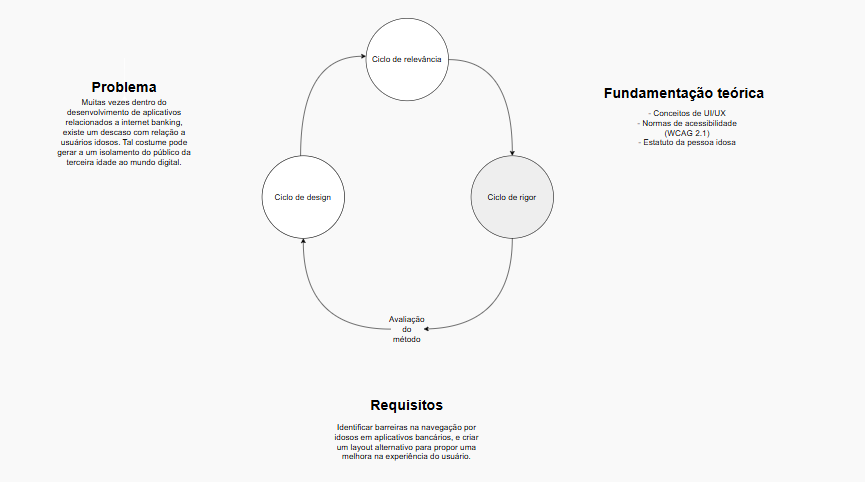
\includegraphics[width=0.85\textwidth]{imagens/dsr-teste} 
    \caption{Estrutura feita em cima do DSR pensando no desenvolvimento de um protótipo para idosos.}
    \label{fig:dsr-teste}
\end{figure}

Conforme é possível ver na figura, existem três processos dentro do DSR. Esses três ciclos principais possuem cada um sua importância, sendo eles: relevância, design e rigor.

Ciclo de relevância: Nesta parte do processo, foi feita uma pesquisa para identificar se realmente há uma necessidade de melhora nos designs de bancos digitais, visto o aumento da digitalização e a dificuldade de acesso do público da terceira idade, criando um "abismo digital". Com uma pesquisa, foram encontrados alguns pontos que reforçaram os motivos de uma mudança no atual cenário. Foi analisado o crescimento nos últimos anos do internet banking, assim como o aumento do número da população idosa no Brasil, que sofre com diversos problemas ao se locomover pelas cidades, tanto físicos quanto de infraestrutura.

Ciclo de Design: Foi realizado um estudo sobre UI/UX para melhorar a experiência do usuário idoso, assim como adotadas regras do WCAG. Foram realizadas entrevistas para descobrir os principais pontos de dificuldade desse grupo, e após o desenvolvimento de um protótipo levando esses pontos em consideração, um teste de usabilidade foi feito.

Ciclo de Rigor: Foram consultadas diretrizes de acessibilidade como o WCAG 2.1 e o Estatuto da Pessoa Idosa (Lei n 10.741). Houve a fundamentação teórica utilizando a interação humano computador (IHC), focando nas limitações da terceira idade, para garantir a funcionalidade do protótipo.

\subsection*{Entrevista}

Procurando descobrir as principais dificuldades do público idoso, foram separadas diversas perguntas, seguindo o padrão ""tal"" (exemplo).

- Pergunta 1: dddsadasasd
- Pergunta 2: dddsadasasd
- Pergunta 3: dddsadasasd
- Pergunta 4: dddsadasasd

\subsection*{Estudo dos dados obtidos}

Após a análise dos dados obtidos pelas entrevistas, foi criado uma tabela com as principais dificuldades relatadas pelos entrevistados e possíveis maneiras de resolvê-las. 

\subsection*{Desenvolvimento de um protótipo}

Com o foco em desenvolvê-lo seguindo o máximo do que é recomendado dentro das normas de design inclusivos apresentadas anteriormente neste trabalho, foi escolhida uma abordagem minimalista. O excesso de itens na tela pode causar confusão ou desanimar o usuário.

\subsection*{Teste de usabilidade}

Após a finalização do protótipo, foi hora de apresentá-lo ao público. Foram sugeridos diversas atividades bancárias para que o usuário fizesse e marcado o tempo que a atividade levou para ser concluída. 

- Atividade 1: sadasdsdads

[Tabela com entrevistados e seus respectivos tempos]

- Atividade 2: dsadsaaddsad

[Tabela com entrevistados e seus respectivos tempos]

- Atividade 3: dsadasddsads

[Tabela com entrevistados e seus respectivos tempos]

Fazendo isso, foi possível verificar se as ações dentro do teste estavam sendo feitas de uma forma dinâmica, comprovando uma melhora no design, atendendo ao público idoso.

\label{sec:proposta}